%--------------------------------------------------------------------
% Эта преамбула с комментариями для написания лабораторных работ по
% физике. В еe основе информация из книги С. М. Львовского "Набор и
% верстка в пакете Latex", а также материалы по курсу "Документы и
% презентации в Latex" от ВШЭ https://www.coursera.org/learn/latex. Ну
% и мой опыт (1 год и 16 лабораторных работ + 2 Вопроса по выбору)
% Автор - Баринов Леонид
% Дата - 06.08.2019
%--------------------------------------------------------------------
%--------------------------------------------------------------------
% Для начала необходимо определиться с типом документа. Оптимальный
% (на мой взгляд) вариант - article. Также существуют типы book,
% report, proc и другие. Также в необязательном аргументе можно
% указать тип страницы и размер шрифта. Стандарт по умолчанию - А4 и
% 12 (иногда 10) шрифт. Необязательный аргумент шрифта может принимать
% только 3 параметра - 10, 11, 12 (pt).

\documentclass[a4paper, 12pt]{article}

%--------------------------------------------------------------------
% Чтобы использовать другие размеры шрифта используется пакет
% extsizes. Он позволяет указывать в \documentclass такие размеры - 8,
% 9, 10, 11, 12, 14, 17, 20 (pt). При указании других размеров могут
% возникать различные проблемы.

\usepackage{extsizes}

%--------------------------------------------------------------------
% Необходимо определиться с кодировкой документа. Идеального варианта
% для русского языка не существует - каждый чем-то немного плох. Для
% особо интересующихся - Приложение И в 5 издании книги Львовского. Я
% воспользовался вариантом, предлагаемым на курсе по Latex от ВШЭ.

\usepackage[T2A]{fontenc}
\usepackage[utf8]{inputenc}

%--------------------------------------------------------------------
% Для соблюдения типографских традиций (оказывается такие существуют)
% различных стран создан пакет babel. Самое заметное его действие -
% latex научиться переносить слова того языка, который вы укажите.
% Можно указать несколько языков через запятую. Основной язык
% документа указывается последним.

\usepackage[english,russian]{babel}

%--------------------------------------------------------------------
% Перейдем к заданию полей документа. Есть несколько способов, но
% самый простой из них - это воспользоваться пакетом geometry, который
% позволяет определить все поля документа (начиная с краев листа, что
% важно, так как некоторые другие способы позволяют это сделать только
% косвенно)

\usepackage{geometry}
\geometry{top=25mm}
\geometry{bottom=35mm}
\geometry{left=35mm}
\geometry{right=20mm}

%--------------------------------------------------------------------
% От полей логично перейти к колонтитулам. Тут нам поможет пакет
% fancyhdr. Для него существует 6 колонтитулов - верхний, левый;
% верхний, по центру; верхний, правый и такие же нижние. По умолчанию
% номер страницы находится снизу по центру, а также существует
% линейка, очерчивающие верхний колонтитул. Мне показалось интересным
% сделать колонтитулы схожие с колонтитулами в лабнике. 

\usepackage{fancyhdr}
\pagestyle{fancy}
\renewcommand{\sectionmark}[1]{\markboth{#1}{}} 
% \renewcommand{\headrulewidth}{0mm} % Если необходимо убрать линейку,
% или изменить ее длину
% \lfoot{} % Нижний левый
% \rfoot{} % Нижний правый
% \rhead{} % Верхний правый
% \chead{} % Верхний в центре
\lhead{\thepage} % Номер страницы в левом верхнем углу
\cfoot{} % Оставить нижний колонтитул без цифры

%--------------------------------------------------------------------
% Самое время научиться работать с формулами. А точнее добавить пакеты
% от Американского математического общества, которые позволять
% пользоваться большим количеством математических символов.

\usepackage{amsmath,amsfonts,amssymb,amsthm,mathtools}

%--------------------------------------------------------------------
% Также очень хочется пользоваться русскими буквами в формулах, для
% этого подключаем пакет mathtext, который добавляет окружение
% \text{}. Внутри него можно писать русские буквы в математическом
% режиме.

\usepackage{mathtext}

%--------------------------------------------------------------------
% Большим преимуществом вашего pdf документа будет возможность поиска
% в нем по словам или буквами. (Например, в Ивановнике это
% невозможно)

\usepackage{cmap}

%--------------------------------------------------------------------
% Куда же в физике без картинок и графиков? Давайте исправим
% эту недоработку

\usepackage{graphicx}
\graphicspath{images/} % Необходимо, если рисунки
% находятся в другой папке

%--------------------------------------------------------------------
% graphicx не позволяет вставлять обтекаемые рисунки, но на
% практике они очень нужны. Для этого существует пакет wrapfig

\usepackage{wrapfig}

%--------------------------------------------------------------------
% latex вставляет рисунки по определенному алгоритму. Его,
% конечно, можно менять, но это не настолько просто. Как
% правило, хочется, чтобы картинка располагалась там, где мы это
% указали в коде. Для этого существует несколько пакетов, один из
% них floatrow. Он позволяет для окружения figure указывать
% необязательный аргумент - H (именно большое h), что на latex'овском
% языке означает: вставить картинку здесь и только здесь. (даже если
% облик документа несколько пострадает)

\usepackage{floatrow}

%--------------------------------------------------------------------
% По правилам оформления рисунок всегда должен быть подписан. Для
% этого существует команда \caption{}. Но обычные настройки caption
% меня не совсем устроили. Хотелось сделать подпись меньше
% основного шрифта, а также слово Рис жирным и использовать
% разделитель точку, а не двоеточие. В этом помогает пакет,
% который называется caption (совпадение?)

\usepackage[margin=10pt,font=small,labelfont=bf,labelsep=period]{caption}

%--------------------------------------------------------------------
% Последним важным пунктом остались таблицы. Ведь куда-то нужно
% заносить результаты измерений. На данный момент во время выполнения
% лабораторных работ я заношу результаты в таблицу excel, а потом с
% помощью сайта www.tablesgenerator.com превращаю в таблицу latex и
% дооформляю.

\usepackage{array,tabularx,tabulary,booktabs}

%--------------------------------------------------------------------
% После excel есть ощущения, что везде объединить колонки или строки
% легко. В latex не совсем так. Помогают пакеты multirow, multicol. 

\usepackage{multirow}
\usepackage{multicol}

%--------------------------------------------------------------------
% Иногда могут потребоваться длинные таблицы на несколько страниц.
% Обычные таблицы latex воспринимает как одну букву. И
% становиться понятно, почему возникают проблемы при переносе
% обычной таблицы. (Ведь нельзя же перенести одну букву!). Поэтому
% вместо обычной таблицы нужна длинная таблица.

\usepackage{longtable}

%--------------------------------------------------------------------
% Часто в таблице хочется сделать перенос текста или формулы. Просто
% так это сделать не получиться из-за синтаксиса tabular. Для этого
% каждый раз необходимо создавать новое окружение tabular, что
% утомительно. Поэтому можно ввести команду \specialcell
% (назвать можно по-любому)
    
\newcommand{\specialcell}[2][c]{%
	\begin{tabular}[#1]{@{}c{}}#2\end{tabular}}

%--------------------------------------------------------------------
% Когда в таблице много колонок и строк, кажется, что они находятся
% слишком близко к друг другу. Можно переопределить
% несколько параметров, чтобы выглядело лучше. Это можно сделать либо
% в преамбуле, либо непосредственно в документе. Первое
% переопределение отвечает за интервал между строками, второе за
% интервал между колонками

% \renewcommand{\arraystretch}{1.8} 
% \renewcommand{\tabcolsep}{1cm} 

%--------------------------------------------------------------------
% В русской типографской традиции принято начинать каждый новый абзац
% с красной строки. Даже первый после заголовка (или подзаголовка).
% Чтобы каждый раз не ставить красную строку вручную существует пакет
% indentfirst

\usepackage{indentfirst}

%--------------------------------------------------------------------
% Некоторые модификаторы начертания

\usepackage{soul}
\usepackage{soulutf8}
 
\begin{document}
\thispagestyle{empty}
\begin{center}
    \textit{Федеральное государственное автономное образовательное\\ учреждение высшего образования }

    \vspace{0.5ex}

        \textbf{«Московский физико-технический институт\\ (национальный исследовательский университет)»}
\end{center}

\vspace{10ex}

\begin{center}
    \vspace{13ex}

    \so{\textbf{Лабораторная работа №_._._}}

    \vspace{1ex}

    по курсу общей физики

    на тему:

    \textbf{\textit{<<>>}}

    \vspace{30ex}

    \begin{flushright}
        \noindent
        \textit{Работу выполнил:}\\  
        \textit{Баринов Леонид \\(группа Б02-827)}
    \end{flushright}
    \vfill
    Долгопрудный \\2019
\newpage
\setcounter{page}{1}
\fancyhead[R]{\nouppercase{\leftmark}}	
\end{center}

\section{Аннотация}
В работе будет наблюдаться резонанс
напряжений в последовательной цепи
переменного тока. 

\section{Теоретические сведения}

Рассмотрим электрическую цепь, состоящую
из резистора $R$ и катушки
индуктивности $L$ 
с импедансом $Z_L = r_L+i\Omega L$,
последовательно подключённых к внешнему
источнику, ЭДС которого меняется по
синусоидальному закону с частотой
$\Omega$ (рис. 1).

\begin{wrapfigure}{r}{0.5\linewidth}
    \vspace{-5ex}
    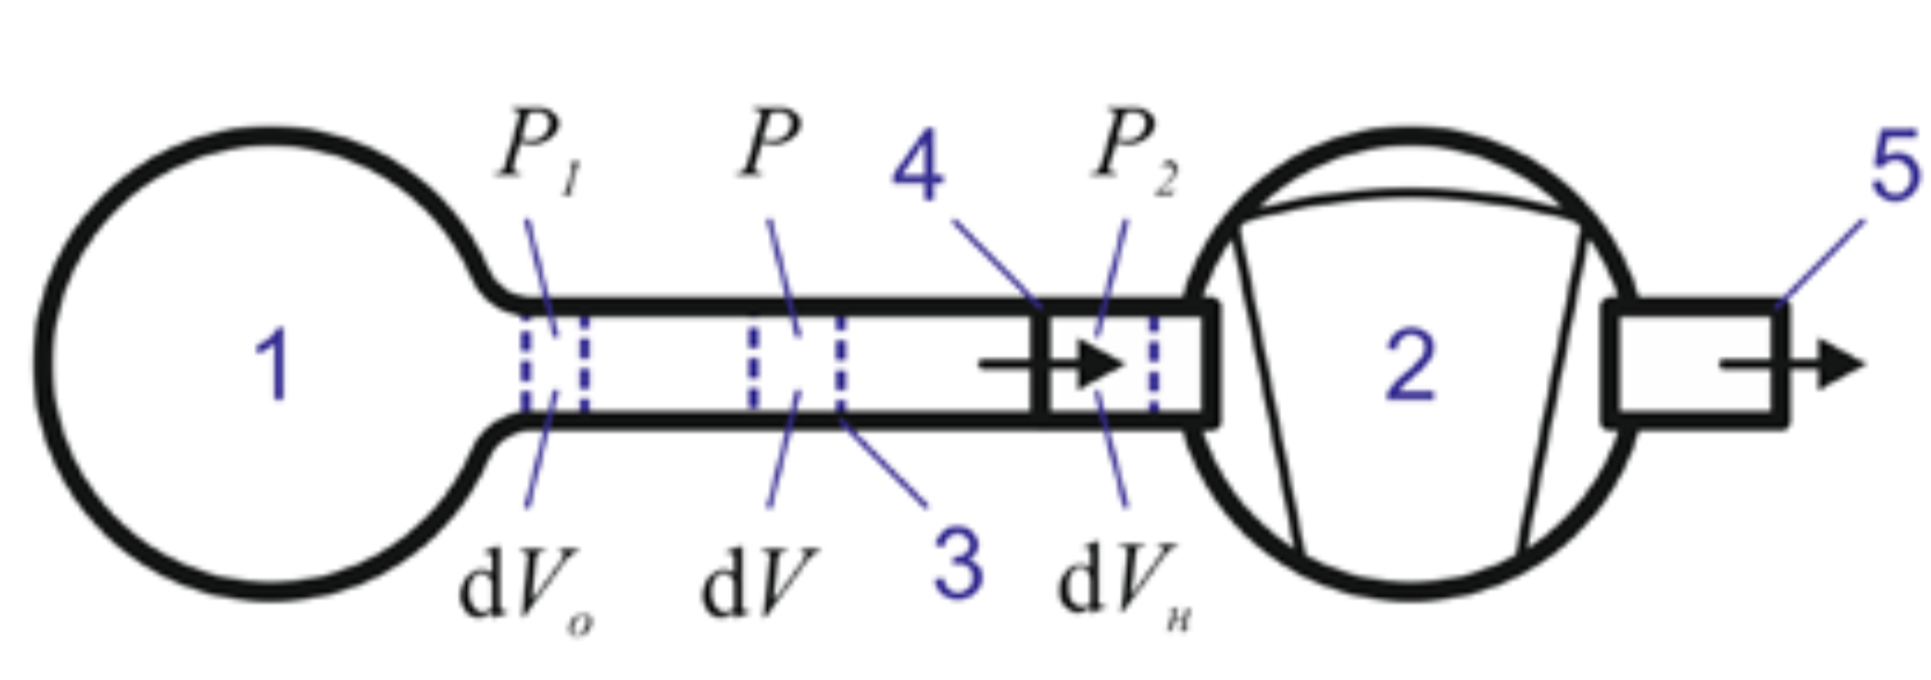
\includegraphics[width=\linewidth]{1}
    \captionsetup{justification=centering}
    \caption{Схема установки для
        изучения закона Ома в цепи
    переменного тока}
\end{wrapfigure}

Обозначим через $U_R$ напряжение на
резисторе, через $U_L$ — напряжение на
катушке и через $U_{R+L}$ — суммарное
напряжение на катушке и на резисторе.
Для этих напряжений справедливы
комплексные соотношения:
\begin{equation}
    \begin{aligned}
    \widehat U_R = \widehat I_R, \quad
    \widehat U_L = \widehat I (r_L +
    i\Omega L)\\
    \widehat U_{R+L} = \widehat I
    (R+r_L + i\Omega L).
\end{aligned}
\end{equation}

Здесь $r_L$ — активное сопротивление
катушки, которое характеризует суммарные
потери энергии в катушке, в том числе
потери в её ферромагнитном сердечнике. 

Переходя к модулям и фазам токов и
напряжений, найдём из (1):
\begin{align}
    & U_R = I \cdot R, & \tg \psi_1 &= 0;
    \\
    & U_L = I \cdot \sqrt{r_L^2+(\Omega
        L)^2}, & \tg \psi_2 &= \frac{\Omega
L}{r_L};\\
    & U_{R+L} = I \sqrt {(R+r_L)^2
    +(\Omega L)^2} , & \tg \psi_3 &=
    \frac{\Omega L}{R + r_L}.
\end{align}

В этих формулах $U$ и $I$ обозначают
эффективные значения напряжений и токов
(показания приборов).

Измеряя с помощью трёх вольтметров
значения $U_R$, $U_L$ и $U_{R+L}$. И зная
сопротивление резистора $R$, нетрудно
вычислить, пользуясь формулами (2), (3)
и (4), силу тока в цепи, активное
сопротивление катушки $r_L$, её
индуктивность $L$, мощность $P_L$, выделяемую
на катушке, и сдвиг фаз между током и
напряжением на катушке. 

Рассчитаем мощность переменного тока,
выделяемую в катушке. Мгновенное
значение мощности равно 
\begin{equation*}
    P = U(t)\cdot I(t).
\end{equation*}
Средняя мощность за период $T$
определяется формулой
\[
    \overline{P} = \frac{1}{T}
    \int\limits_0^T U(t) \cdot I(t) dt
\]
Полагая $I(t) = I\sqrt{2}\cos\Omega t$,
$U(t) = U\sqrt{2} \cos (\Omega t +
\psi)$, получим после интегрирования:
\begin{equation}
    \overline P_L = U_L \cdot I \cos
    \psi = I^2 \cdot r_L
\end{equation}
Средняя мощность, выделяющаяся в катушке
самоиндукции, определяется, таким
образом, действительной частью её
импеданса.

Активное сопротивление катушки $r_L$ можно
определить, если включить её в
последовательный колебательный контур с
известными параметрами — сопротивлением
$R$ и ёмкостью $C$ (рис. 2). В контуре,
настроенном в резонанс на частоту
$\Omega$ 
внешнего источника (собственная частота
контура и внешняя совпадают: $\omega =
\Omega$),
реактивные сопротивления индуктивности и
ёмкости одинаковы:
\begin{equation}
    \omega_0 L = \frac{1}{\omega_0 C}.
\end{equation}

Определив каким-либо экспериментальным
способом добротность $Q$ этого контура,
можно рассчитать полное сопротивление
контура $R_\Sigma$ в резонансе, поскольку
\begin{equation}
    Q = \frac{\omega_0 L}{R_\Sigma} =
    \frac{1}{\omega_0 C R_\Sigma}
\end{equation}

Резонансное сопротивление контура
$R_\Sigma$
включает в себя известное сопротивление
резистора $R$ и активное сопротивление
катушки $r_L$:
\begin{equation}
    R_\Sigma = R + r_L .
\end{equation}

\section{Оборудование}
\textbf{В работе используются:}
регулировочный автотрансформатор,
катушка индуктивности с выдвижным
сердечником, магазин емкостей,
резисторы, амперметр, три вольтметра,
ваттметр, осциллограф, универсальный
мост.
\subsection*{Экспериментальная установка}
Схема установки для исследования закона
Ома в цепи переменного тока представлена
на рис. 1. Цепь, состоящая из резистора
$R_1 \simeq 100\ \text{Ом}$ и катушки $L$ с выдвижным
сердечником, подключена к
автотрансформатору, выходное напряжение
которого можно менять от 0 до 127 В.
Напряжения на каждом из элементов и
суммарное напряжение цепи измеряются
тремя вольтметрами: $V_R$, $V_L$ и
$V_{R+L}$·
Амперметр $A$ измеряет ток в цепи, а
ваттметр $P$ — мощность, выделяющуюся на
катушке.

\begin{wrapfigure}[20]{r}{0.5\linewidth}
    \vspace{3ex}
    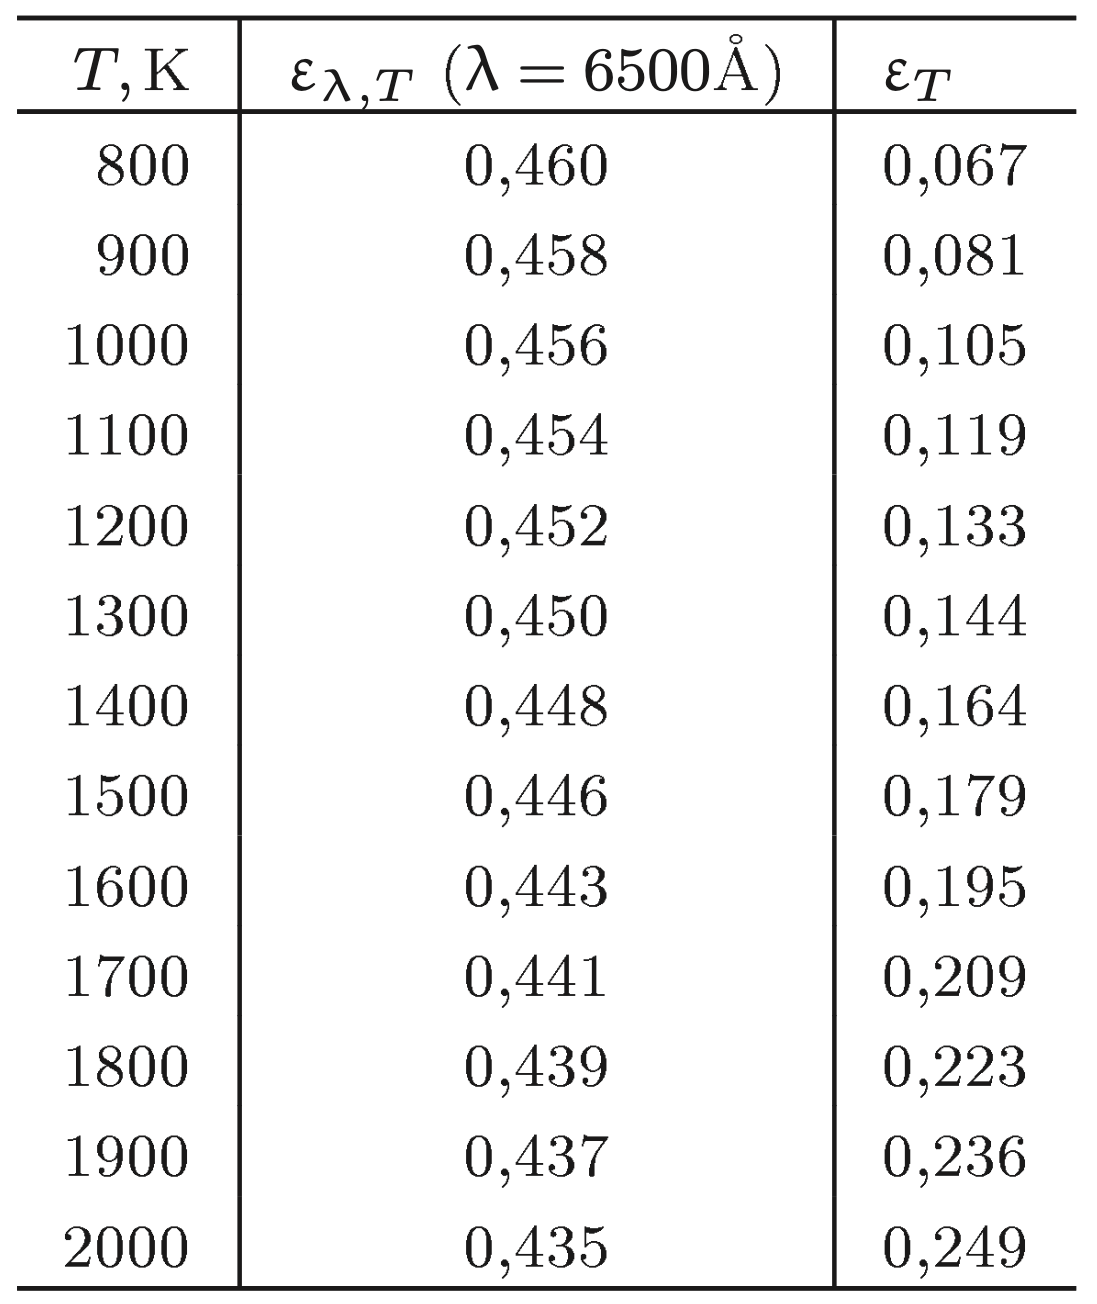
\includegraphics[width=\linewidth]{2}
    \captionsetup{justification=centering}
    \caption{Схема установки для
    наблюдения резонанса напряжений.}
\end{wrapfigure}

Ваттметр электродинамической системы
состоит из двух катушек, одна из которых
вращается в магнитном поле другой, если
через них течёт ток. Токовая катушка
ваттметра $II^*$ включается последовательно
в исследуемую цепь, а катушка напряжений
(потенциальная) $VV^*$ — параллельно к
элементу, в котором измеряется
выделяемая мощность.

Предел измерений
устанавливается при помощи
переключателей или штепселей, которые
вставляются в соответствующие гнёзда:
произведение цифр против штепселя
токовой катушки $II^*$ и против
переключателя катушки напряжений $VV^*$
определяет мощность, соответствующую
отклонению стрелки на всю шкалу. Отсчёт
мощности ведётся по любой из шкал,
обозначенных буквой $P$.

Схема установки для изучения резонанса
напряжений изображена на рис. 2.
Последовательно соединены резистор $R_2
\approx 5\ \text{Ом}$, катушка $L$ и
магазин емкостей $C$.
Амперметр $A$ измеряет ток в цепи,
вольтметр $V_c$ — напряжение на ёмкости,
вольтметр $V_\Sigma$ — суммарное напряжение на
контуре. Резонанс можно зафиксировать с
помощью осциллографа, если подать на
вход $X$ напряжение с контура, а на вход
$Y$ — напряжение с резистора $R_2$,
пропорциональное току в цепи. В общем
случае на экране виден эллипс. При
резонансе эллипс вырождается в прямую
линию.

Резонансные напряжения на контуре
$U_{\Sigma, \text{рез}}$,
и на ёмкости $U_{c, \text{рез}}$, рез равны
соответственно
\begin{equation}
    U_{\Sigma, \text{рез}} =
    I_{\text{рез}} =
    \frac{I_\text{рез}}{\Omega C}.
\end{equation}
Сравнивая (7) и (9), получим 
\begin{equation}
    Q = \frac{U_c, \text{рез}}{U_\Sigma,
    \text{рез}}
\end{equation}

Формула (10) показывает, что добротность
контура может быть найдена по измеренным
значениям напряжений на контуре и на
конденсаторе при резонансе. Зная
добротность контура и ёмкость $C$, можно
рассчитать $R_\Sigma$ по формуле (7), а затем
определить $r_L$.

\section{Результаты измерений и обработка результатов}

Снимем зависимости тока $I$, напряжений
$U_R$, $U_L$, $U_{R+L}$ и мощности $P_L$
от координаты сердечника $x$. Вычислим
активное сопротивление катушки $r_L$ по
формуле (5), а затем определим $L$,
исходя из формулы (3)

Сопротивление реостата:
\[
    R_1 = 98 \pm 2\ \text{Ом}
\]

\renewcommand{\arraystretch}{1.2} 
\begin{table}[H]
\centering
\begin{tabular}{|c|c|c|c|c|c|c|c|}
\hline
$I, \ \text{А}$    & $U_R, \ \text{В}$ &
$U_L, \ \text{В}$& $U_{R+L}, \ \text{В}$
& $P_L, \ \text{Вт}$   & $x, \
\text{мм}$  & $r_L, \ \text{Ом}$    & $L,\
\text{мГн}$    \\ \hline
0,50 & 43 & 102 & 113 & 14,50 & 5  & 58,00 & 622,87 \\ \hline
0,55 & 49 & 98  & 103 & 14,00 & 7  & 46,28 & 547,98 \\ \hline
0,63 & 54 & 94  & 111 & 13,25 & 9  & 33,92 & 466,64 \\ \hline
0,65 & 59 & 91  & 111 & 13,00 & 11 & 30,77 & 434,96 \\ \hline
0,70 & 62 & 88  & 110 & 12,50 & 13 & 25,51 & 392,03 \\ \hline
0,73 & 65 & 85  & 109 & 12,00 & 15 & 22,83 & 366,23 \\ \hline
0,75 & 67 & 82  & 108 & 11,75 & 17 & 20,89 & 341,78 \\ \hline
0,78 & 69 & 80  & 107 & 11,50 & 19 & 19,15 & 323,04 \\ \hline
0,80 & 71 & 78  & 107 & 11,25 & 21 & 17,58 & 305,42 \\ \hline
0,80 & 73 & 76  & 107 & 11,00 & 23 & 17,19 & 297,56 \\ \hline
0,83 & 74 & 74  & 106 & 10,75 & 25 & 15,79 & 281,20 \\ \hline
0,85 & 74 & 71  & 105 & 10,50 & 27 & 14,53 & 261,96 \\ \hline
0,85 & 75 & 70  & 105 & 10,25 & 29 & 14,19 & 258,35 \\ \hline
0,88 & 76 & 69  & 104 & 10,25 & 31 & 13,39 & 247,49 \\ \hline
0,88 & 77 & 67  & 104 & 10,00 & 33 & 13,06 & 240,28 \\ \hline
0,88 & 78 & 66  & 104 & 10,00 & 35 & 13,06 & 236,59 \\ \hline
0,90 & 79 & 65  & 104 & 10,00 & 37 & 12,35 & 226,62 \\ \hline
0,90 & 79 & 64  & 103 & 10,00 & 39 & 12,35 & 223,03 \\ \hline
0,90 & 80 & 63  & 103 & 10,00 & 40 & 12,35 & 219,44 \\ \hline
\end{tabular}
\captionsetup{justification = centering}
\caption{Зависимость тока $I$, активного
сопротивления катушки  $r_L$,
индуктивности катушки  $L$, напряжений
 $U_R$, $U_L$, $U_{R+L}$ и мощности
 $P_L$ от координаты сердечника $x$}
\end{table}

Построим графики зависимостей $L$ и
$r_L$ от положения сердечника и
определим по ним значения $L$ и $r_L$,
соответствующие среднему (резонансному)
положению сердечника.

\[
    r_L = 18 \pm 1 \ \text{Ом}
\]
\[
    L = 310 \pm 30 \ \text{мГн}
\]

Для среднего положения
сердечника построим векторную диаграмму
напряжений
при горизонтальном расположении $U_R$.

Отложим на диаграмме активную ($U_{L, \
\text{акт}}$)
и реактивную ($U_{L, \
\text{реакт}}$) составляющие
напряжения на катушке и рассчитаем по
ним значения $L$ и $r_L$.
\[
    L = 318 \pm 14\ \text{мГн}
\]
\[
    r_L = 2,6 \pm 0,2\ \text{Ом}
\]

\begin{figure}[H]
    \centering
    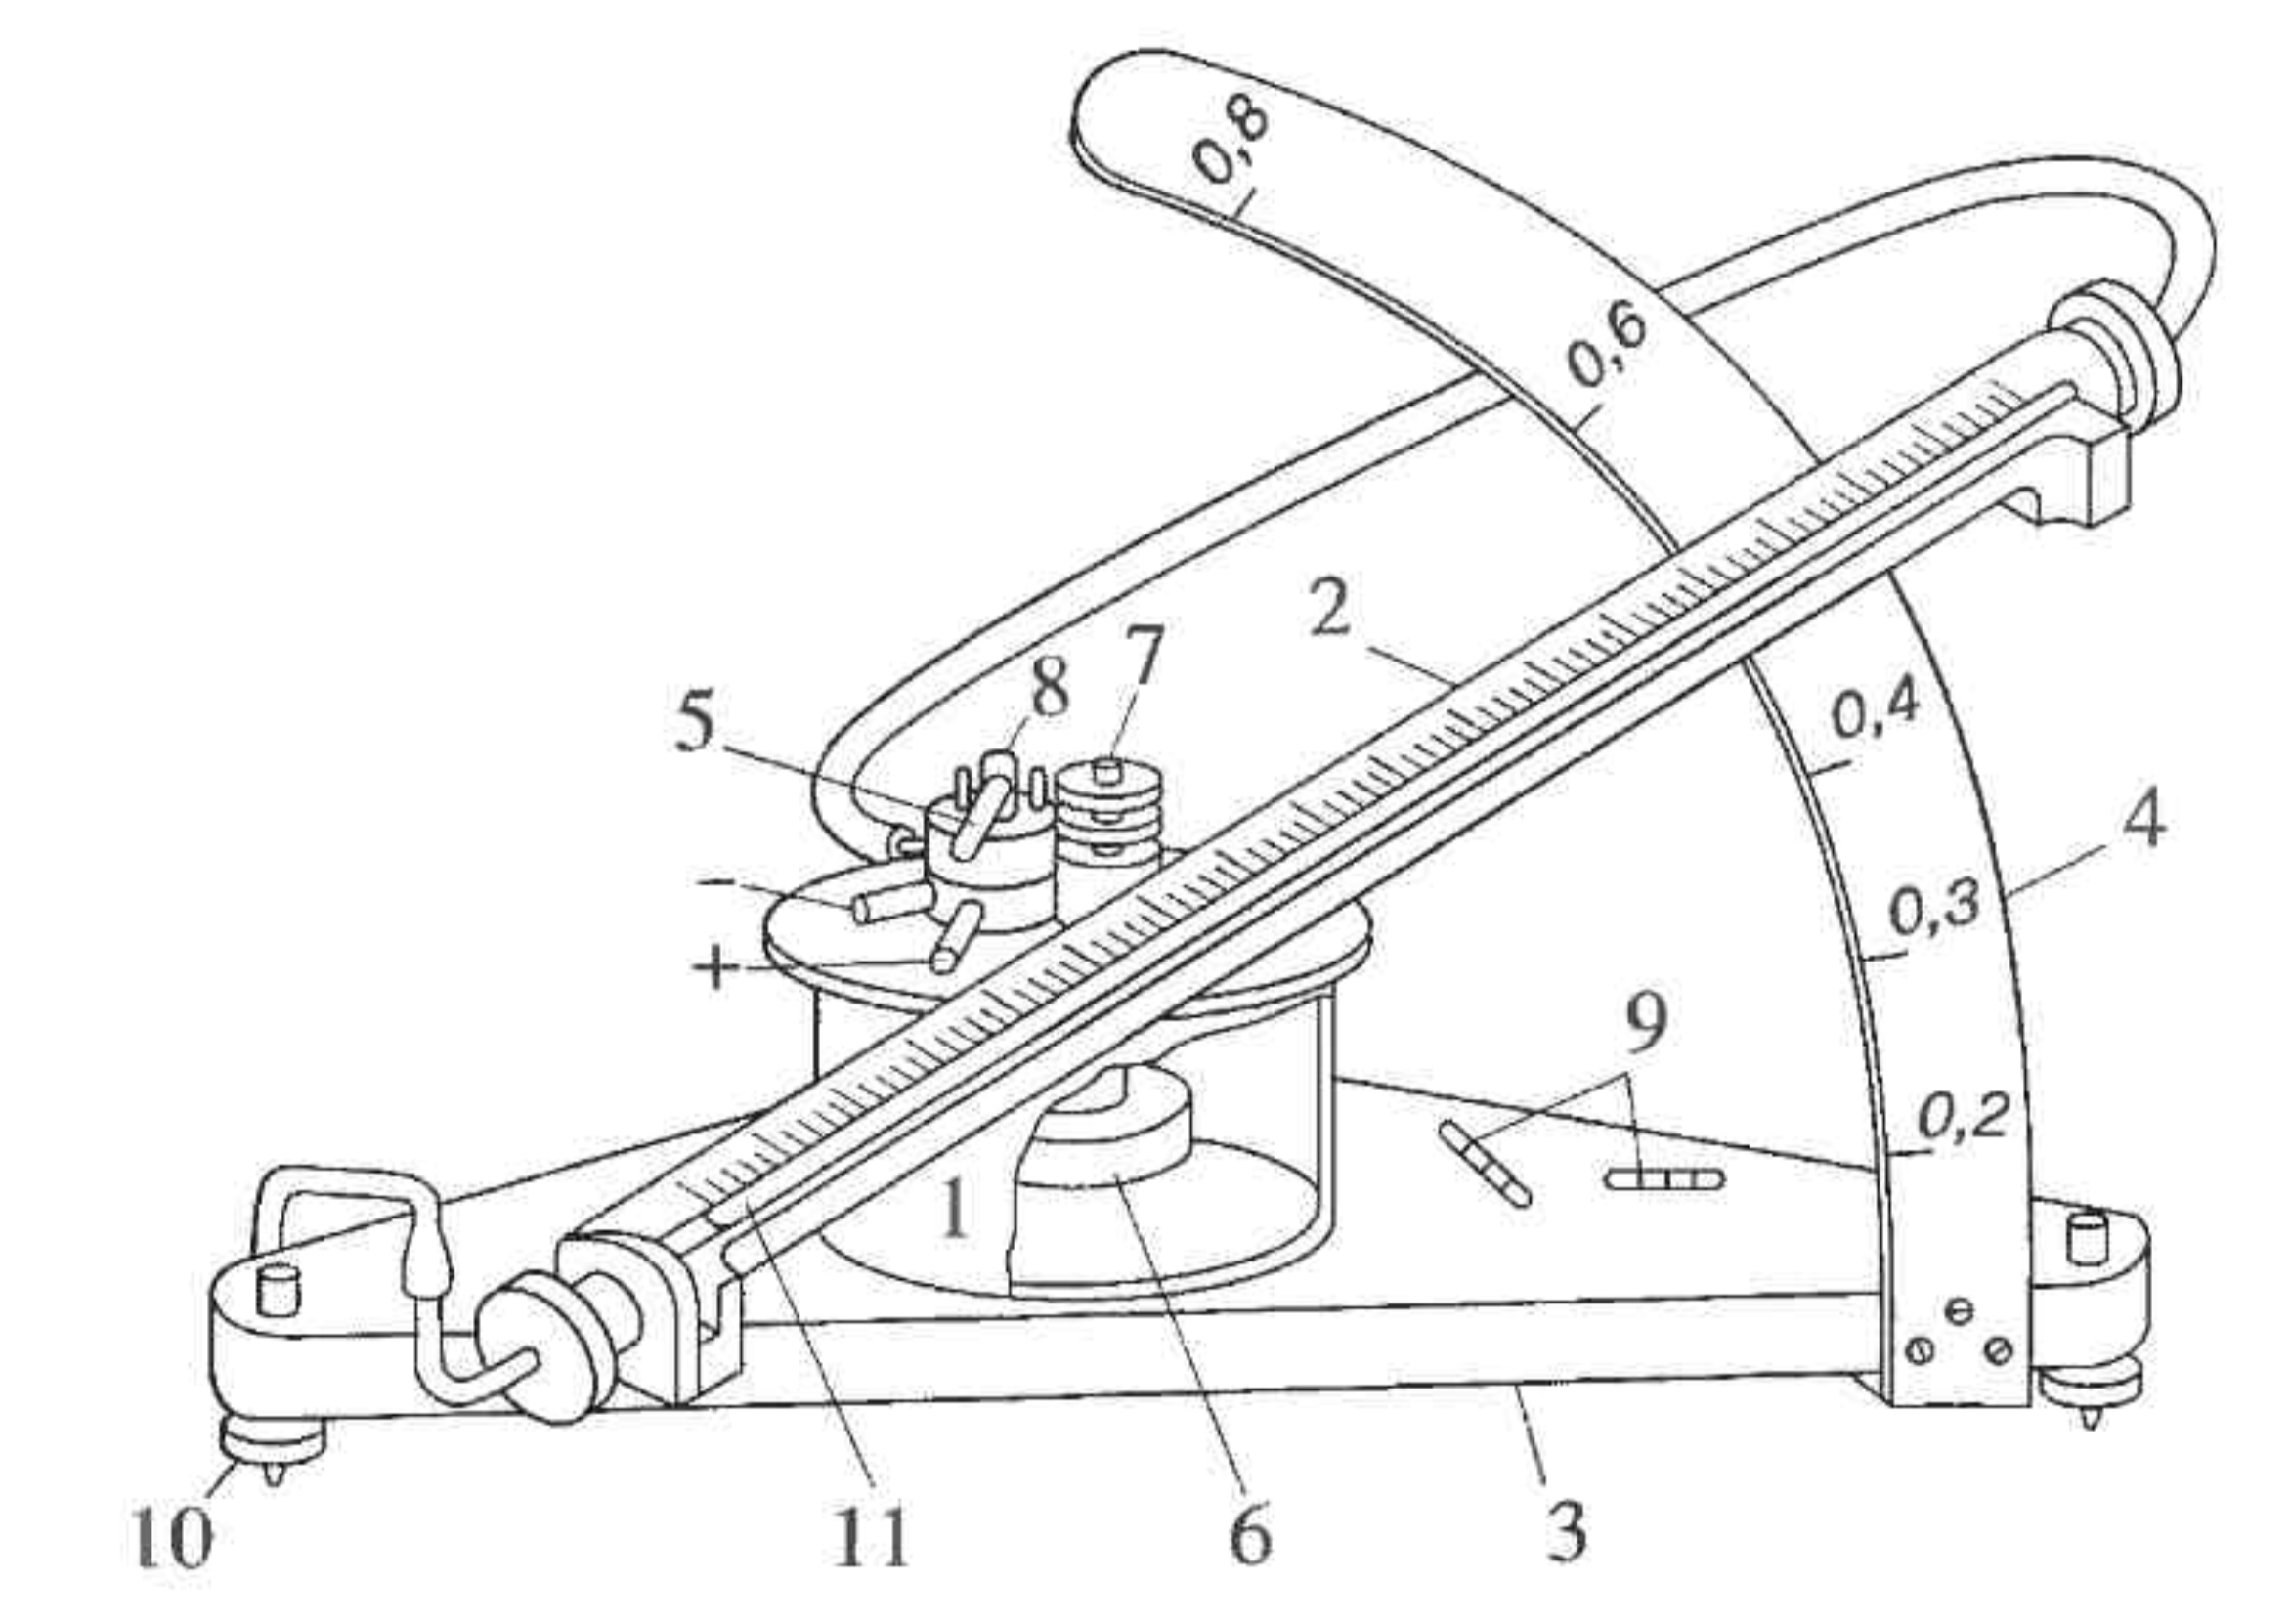
\includegraphics[width=\linewidth]{3}
    \captionsetup{justification=centering}
    \caption{Графики
    зависимостей индуктивности $L$ и
активного сопротивления катушки $r_L$ от
положения сердечника $x$}
\end{figure}

\begin{figure}[H]
    \centering
    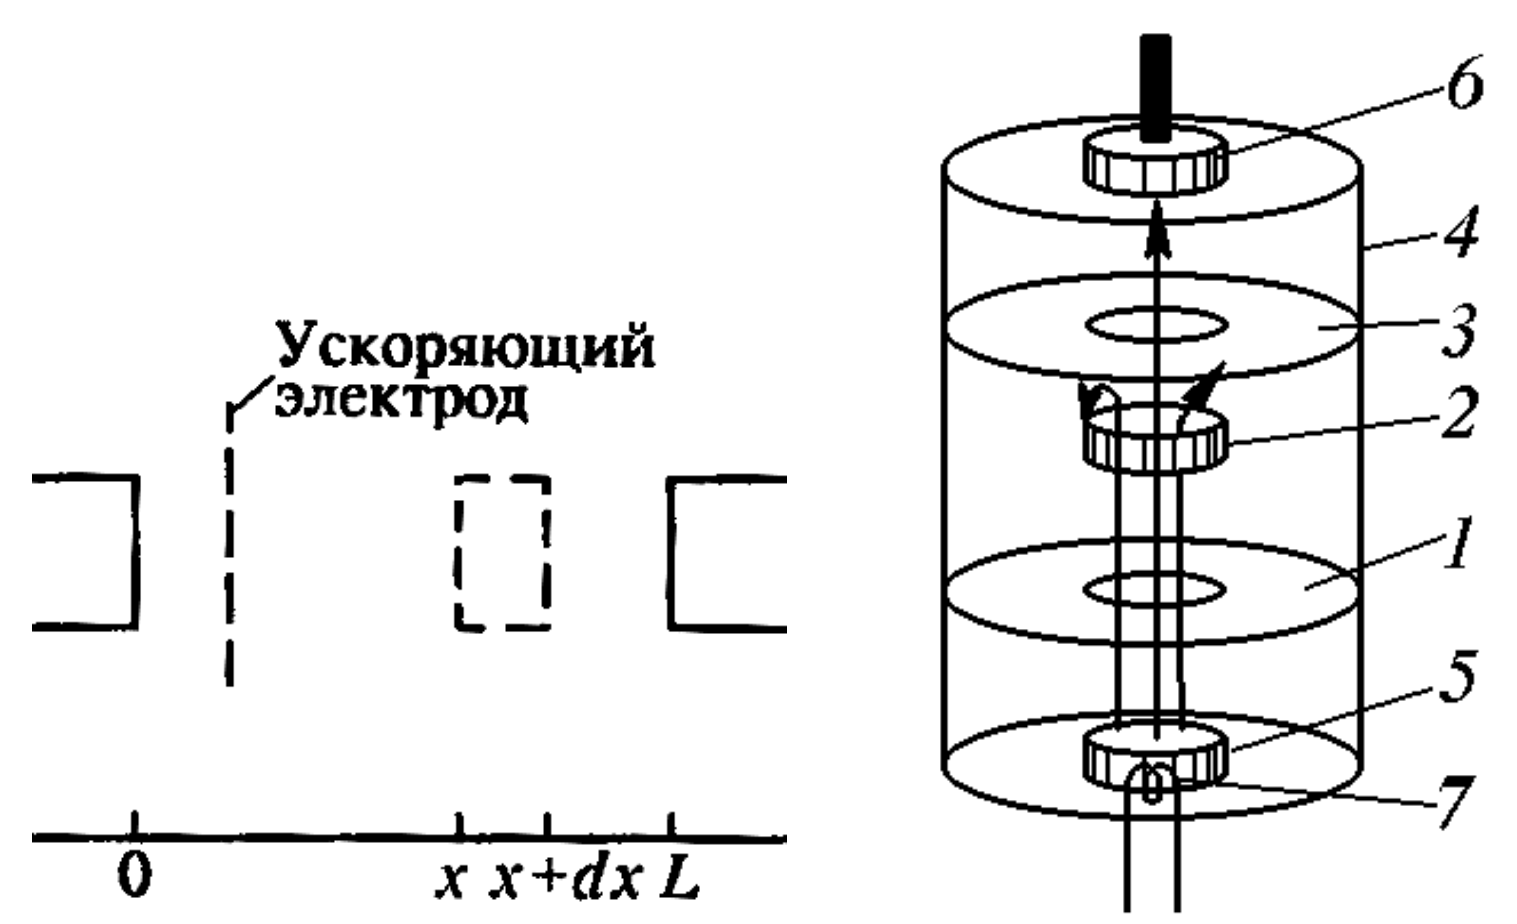
\includegraphics[width=0.6\linewidth]{4}
    \captionsetup{justification=centering}
    \caption{Векторная диаграмма
    напряжений для среднего положения
сердечника}
\end{figure}

Определим по диаграмме $\cos\Theta$ --
сдвиг фаз между током и напряжением на
катушке. Также вычислим значение по
формуле (5)

\[
    \cos\Theta = 0,026 \pm
    0,002 \ (\text{из диаграммы})
\]

\[
    \cos\Theta = 0,180 \pm 0,007 \
    (\text{по формуле (5)})
\]


С помощью векторной диаграммы по теореме
косинусов выразим мощность $P_L$,
выделяемую на катушке, через напряжения
$U_R$, $U_L$, $U_{R+L}$ и сопротивление
$R_1$.

\begin{multline*}
   P_L = U_L I \cos\Theta = U_L
   \frac{U_R}{R_1}\frac{U_{L, \
   \text{акт}}}{U_L} =
   \frac{U_R}{R_1}(U_{L+R}\cos\varphi-U_R)
   = \\
   =
   \frac{U_R}{R_1}
   (U_{L+R}\frac{U_R^2+U_{L+R}^2-U_L^2}{2U_R
       U_{L+R}} - U_R) =
       \frac{U_{L+R}^2-U_R^2-U_L^2}{2 R_1}
\end{multline*}
   
\[
    P_L = 1,65 \pm 0,05 \ \text{Вт}
\]

Значение, измеренное ваттметром:
\[
    P_L^* = 11,3 \pm 0,3 \ \text{Вт}
\]

В схеме, собранной по рис. 2, меняя
емкость, настраиваем контур в резонанс с
частотой сети. Снимем значения
резонансного тока $I$, резонансного
напряжения на емкости $U_c$,
резонансного напряжения на контуре
$U_\Sigma$ и резонансное значение
ёмкости.

Величина дополнительного сопротивления
$R_2$:
 \[
     R_2 = 5,6 \pm 0,1 \ \text{Ом}
\]

\begin{table}[H]
    \begin{tabular}{|c|c|c|c|c|}
        \hline
        $x,\ \text{мм}$ & $I, \
        \text{А}$ & $U_c, \ \text{В}$ &
        $U_\Sigma, \ \text{В}$ & $C, \
        \text{мкФ}$ \\ \hline
        9 & 1,5 & 218 & 25,5 & 20,2\\
        \hline
    \end{tabular}
    \captionsetup{justification=centering}
    \caption {Величины, измеренные во
    время резонанса}
\end{table}

Рассчитаем активное сопротивление
катушки $r_L$ через ток и напряжение на
контуре:
\[
r_L = \frac{U_\Sigma}{I} - R_2
\]

\[
    r_L = 11,4 \pm 0,4 \ \text{Ом}
\]

Рассчитаем $r_L$ и $L$ через добротность
$Q$:
 \begin{align*}
     Q &= \frac{U_c}{U_\Sigma} & Q &= 8,5 \pm 0,2\\
     L &= \frac{1}{\omega_0^2C} =
     \frac{1}{\Omega^2C} & L &= 500 \pm
     30 \ \text{мГн}\\
     r_L &= \frac{\omega_0 L}{Q} - R_2 &
     r_L &= 12,9 \pm 0,9 \ \text{Ом}
\end{align*}

Измерим индуктивность катушки $L$ и ее
активное сопротивление $r_L$ с помощью
моста E7-8 при заданной частоте:
\begin{table}[H]
    \begin{tabular}{|c|c|c|}
        \hline
        $\nu, \ \text{Гц}$ & $L,\
        \text{мГн}$ & $r_L, \ \text{Ом}$
        \\ \hline
        100 & 372 & 13,9\\ \hline
        1000 & 338 & 190,3 \\ \hline
    \end{tabular}
    \captionsetup{justification=centering}
    \caption{Измерение индуктивности $L$
    и активного сопротивления $r_L$ с
помощью моста  E7-8 }
\end{table}

Измерение сопротивления катушки с
помощью омметра:
\[
    r_L = 4,28 \pm 0,05 \ \text{Ом}
\]


\section{Обсуждение результатов и выводы}
Результаты измерений занесены в таблицу
3.
\begin{table}[H]
    \begin{tabular}{|c|c|c|c|c|c|c|}
        \hline
        & Омметр & Мост E7-8 & График &
        Вект. диагр. & $f(I, U_\Sigma)$
                     & $f(Q)$ \\ \hline
        $r_L, \ \text{Ом}$ & $4,28\pm
        0,05$ & $13,9 \pm 0,1$ & $18
        \pm 1$ & $2,6 \pm 0,2$ & $11,4 \pm
        0,4$ & $12,9\pm 0,9$ \\ \hline
        $L, \ \text{мГн}$ & -- & $372 \pm 5$ & $310 \pm
        30$ & $318 \pm 14$ & -- & $500
        \pm 30$ \\ \hline
    \end{tabular}
    \captionsetup{justification =
    centering}
    \caption { Результаты измерений
    активного сопротивления $r_L$ и
индуктивности $L$ различными способами}
\end{table}

Значения достаточно сильно различаются из-за способа измерения
величин. Реальную катушку можно
заменить колебательным контуром с
собственными параметрами: $L$ --
истинное значение индуктивности, $C_L$
-- емкость, $r_L$ -- активное
сопротивление. В результате в этом
контуре возникают колебания с
собственной частотой $\omega_L$. Поэтому
величины, которые мы измеряем в цепи
переменного тока могут заметно
отличаться от величин,
измеренных с помощью приборов,
подключенных непосредственно к катушке.


\end{document}
